\input assets/cs-pre
\bibliography{assets/references.bib}

\begin{document}
\MYTITLE{CMPSC 383: Multi-Agent and Robotic Systems}{Final Project Progress Report}
\MYHEADERS{}

\section{Introduction}
    \textit{Flocking}, in the context of multi-agent systems, involves the collective behavior of a group of interacting, mobile agents. Flocking patterns are exhibited by such a group when the individual agents attempt to move together with their neighbors. This behavior in multi-agent systems mimics the similar flocking behaviors of groups of animals such as birds or fish. Applications of this type of behavior are diverse: multi-robot teams can use flocking to coordinate their movement towards a goal while maintaining a consistent formation or level of proximity~\cite{saska2014swarms,min2011design}, finding optimized solutions to mathematical problems~\cite{cui2009boid}, and simulating the behavior and appearance of flocks or swarms of animals.% TODO: more examples
    \par Boids particular simulation model for multi-agent flocking behaviour~\cite{hartman2006autonomous}. It was first described by Craig Reynolds in 1987~\cite{reynolds1987flocks}. Boids uses a set of three rules for the manipulation: separation, cohesion, and alignment~\cite{reynolds1987flocks,hartman2006autonomous}. More detail on this model can be found in~\Cref{boids}. This model has been used in a number of computer graphics applications, including motion pictures and video games, as well as in robotics applications~\cite{saska2014swarms,min2011design}.
    \par Our project is an implementation of this Boids simulation. To do so, we used the Haskell programming language, a purely functional language with lazy evaluation. This document describes some particulars of Haskell and how they relate to the task of agent programming, the details of the mechanism of our implementation, and the results we acquired from our implementation.

\section{Method}
\subsection{Language Choice}

We chose Haskell as the implementation language for our Boids simulation.
Haskell is a purely functional language with lazy evaluation~\cite{hudak1994haskell,jones2003haskell}. It has been observed that Haskell supports the rapid prototyping of software systems, allowing working systems to be implemented quickly and with minimal complexity~\cite{hudak1994haskell}. The functional programming paradigm in general has been noted to support modularity and allow problems to be decomposed easily~\cite{hughes1989functional}. These observations, along with our previous experience in the language, influenced our choice of Haskell as a platform for our project.

As our class experience with implementing multi-agent simulations has been solely through the object-oriented programming (OOP) paradigm, our language choice presented a challenge, but also a valuable learning experience. Our
implementation of the Boid agents involves the definition of an abstract data
type, which contains the position, velocity, and neighborhood radius of an
individual boid. In Haskell, this is defined as follows:
\begin{listing}[h!]
\begin{minted}{haskell}
data Boid = Boid { position :: Point
                 , velocity :: Vector
                 , radius   :: Float
                 }
\end{minted}
\end{listing}
\FloatBarrier
Note that Haskell, as a purely functional programming language, does not allow mutation of existing values. Therefore, once a
\mintinline{haskell}|Boid| is created, it cannot be mutated, and updating the \mintinline{haskell}|Boid|'s state
requires the creation of an entirely new \mintinline{haskell}|Boid| instance.

Also, in contrast to a corresponding OOP implementation, which might define some \mintinline{haskell}|Boid|behaviour (i.e. methods) to accompany this basic data structure, this \mintinline{haskell}|Boid| data type is kept distinct from the functions which act upon it.. Instead, we define a type called \mintinline{haskell}|Update|:

\begin{minted}{haskell}
type Update = Boid -> Boid
\end{minted}

Thus, a function of type \mintinline{haskell}|Update| is a function that takes a \mintinline{haskell}|Boid| and returns
a new \mintinline{haskell}|Boid|. We use \mintinline{haskell}|Update| to define \mintinline{haskell}|Behaviour|:

\begin{minted}{haskell}
type Perception = [Boid]
type Behaviour = Perception -> Update
\end{minted}

This defines a \mintinline{haskell}|Behaviour| as a function that maps an agent's perception of its environment (in this case, a \mintinline{haskell}|Boid|'s visible neighborhood) to
a function for updating its environment. These examples demonstrate how implementing a multi-agent
simulation in a purely-functional language requires a different conception of
what it means programmatically for an Agent to behave. 

\subsection{Boids}\label{boids}

Boids models the behaviour of a flock in as being effected by three primary steering forces: \textit{cohesion}, the tendency of an individual to stay close to the centre of the flock; \textit{separation}, the tendency of an individual to avoid collision with other individuals, and \textit{alignment}, the tendency of an individual to match velocities with its neighbors~\cite{hartman2006autonomous,reynolds1987flocks}. Each of these steering forces is modeled as a vector, which are then summed to compute the position of a given boid at each time interval.

The separation steering vector $\vec{s}_i$ for a given boid $b_i$ may be calculated as the negative sum of the position vector of $b_i$ and each visible boid $b_j$, using the following formula:

\[ \vec{s}_i = - \sum\limits_{\forall b_j \in V_i} (p_i - p_j) \]

where $V_i$ is the set of boids visible by $b_i$ (i.e. the neighborhood)~\cite{hartman2006autonomous}. In our implementation, this formula corresponds to the following Haskell source code:

\begin{minted}{haskell}
separation :: Boid -> Perception -> Vector
        -- :: Boid -> [Boid] -> V3 Float
separation self neighbors =
    let p = position self
    in sumV . map (^-^ p) $ positions neighbors
\end{minted}

The cohesion steering vector $\vec{k}_i$ for a given boid $b_i$ may be calculated by finding the centre of density $c_i$ of the visible boids $V_i$ using the formula

\[ c_i = \sum\limits_{\forall b_j \in V_i} \frac{p_j}{m} \]

where $m$ is the cardinality of $V_i$. The steering vector may then be calculated by subtracting $b_i$'s position from $c_i$~\cite{hartman2006autonomous}:

\[ \vec{k}_i = c_i - p_i \]

In our implementation, these formulae corresponds to the following Haskell source code:

\begin{minted}{haskell}
centre :: Perception -> Vector
    -- :: [Boid] -> V3 Float
centre boids =
    let m = fromIntegral $ length boids :: Float
    in sumV $ map (^/ m) $ positions boids

cohesion :: Boid -> Perception -> Vector
      -- :: Boid -> [Boid] -> V3 Float
cohesion self neighbors =
    let p = position self
    in centre neighbors - p
\end{minted}

Finally, the alignment steering vector $\vec{m}_i$ for a boid $b_i$ may be calculated by averaging the velocities of the set of visible boids $V_i$ using the following formula

\[ \vec{m}_i = \sum\limits_{\forall b_j \in V_i} \frac{\vec{v}_j}{m} \]

where $\vec{v}_j$ is the velocity of $b_j$. If the cardinality of $V_i$ is zero, then $\vec{v}_i = 0$~\cite{hartman2006autonomous}. In our implementation, this formula corresponds to the following Haskell source code:

\begin{minted}{haskell}
alignment :: Boid -> Perception -> Vector
       -- :: Boid -> [Boid] -> V3 Float
alignment _ []        = V3 0 0 0
alignment _ neighbors =
    let m = fromIntegral $ length neighbors :: Float
    in (sumV $ map velocity neighbors) ^/ m
\end{minted}

Once all three steering vectors have been calculated, they are combined to find the velocity $\vec{v_i\prime}$ of a boid

\[ \vec{v_i\prime} = \vec{v_i} + S.\vec{s_i} + K.\vec{k_i} + M.\vec{m_i} \]

where $S$, $K$, and $M$ are coefficients which control the weight of each steering force and are typically global parameters to the simulation.

The position of that boid at time $t + \Delta t$ maythen  be updated using $\vec{v_i\prime}$

\[ p\prime_i = p_i + \Delta t\vec{v_i}\]

In our implementation, these formulae corresponds to the following Haskell source code:

\begin{minted}{haskell}
steer :: Weights -> Behaviour
   -- :: Weights -> [Boid] -> Boid -> Boid
steer (s, c, m) neighbors self =
    let s_i  = s *^ separation self neighbors
        c_i  = c *^ cohesion self neighbors
        m_i  = m *^ alignment self neighbors
        v'   = velocity self ^+^ s_i ^+^ c_i ^+^ m_i
        p    = position self
        p'   = p ^+^ v'
    in self { position = p', velocity = v'}
\end{minted}

\subsection{Program Usage}

Our implementation supports a number of command-line arguments to set simulation parameters and control the resulting visualization. The following options for controlling the simulation parameters are supported:

\begin{description}
    \item[Height] of the space can be set using the options \texttt{-x HEIGHT} or \texttt{--height=HEIGHT}. 
    \item[Width] of the space can be set using the options \texttt{-y WIDTH} or \texttt{--width=WIDTH}.
    \item[Number of Boids] can be  set using the options \texttt{-n BOIDS} or \texttt{--num=BOIDS}.
    \item[Boid visibility radius] can be set using the options \texttt{-v RADIUS} or \texttt{--visibility=RADIUS}. The default is 50.
    \item[Simulation speed] can be set using the options \texttt{-p SPEED} or \texttt{--speed=SPEED}. This value sets a coefficient by which the movement vector of each boid is divided every simulation tick. The default is 1000 at 30 frames per second.
\end{description}

Additionally, our implementation allows the user to select one of a set of preset behavior types. These control the values of the weight constants for the three boid steering forces, as discussed in \Cref{boids}.

\begin{description}
    \item[Equal-Weight Behavior] selected with the command-line flag \texttt{-e} or \texttt{--equal}, sets all weight coefficients to 1.
    \item[Cohesive Behavior] selected with the flag \texttt{-c} or \texttt{--cohesive}, sets weights as follows: $S = 1, K = 0.5, M = 0.5$.
    \item[Swarming Behavior] selected with the flag \texttt{-s} or \texttt{--swarm}, sets the alignment coefficient ($M$) equal to zero, creating true swarming behavior.
\end{description}

Our program may also be run in `debug mode,' using the \texttt{-d} or \texttt{--debug} option. In debug mode, the program will run the visibility radius and velocity vector of each boid, so that the user can gain a greater understanding of how the simulation functions. Finally, the \texttt{-h} or \texttt{--help} flag will print out a summary of the available command-line options.

\section{Results}
    
    The results of this simulation are visible in the following figures:
    \begin{itemize}
        \item Figure~\ref{fig:no-debug} demonstrates our simulation without our ``debug-mode''. Of course, as a static image without any representation of boid vectors, it is difficult to tell how the swarm is behaving.
        \item Figure~\ref{fig:eqweight} demonstrates our ``debug mode'' with equal weights for cohesion, separation, and alignment. A large degree of agent clustering is visible.
        \item However, with smaller radii as in Figure~\ref{fig:eqweight-small}, we see a significantly decreased level of clustering of the agents.
        \item On the other hand, increasing the radii as in Figure~\ref{fig:eqweight-large}, gives an even greater degree of clustering than before.
        \item With our ``cohesive'' mode, as in Figure~\ref{fig:eqweight-large}, we see that the boids form a much more even distribution throughout the space. This is due the fact that the separation impulse is still present, but does not dominate the vectors of the boids, preventing them from separating a great distance apart.
    \end{itemize}
    
    \begin{figure}
        \centering
        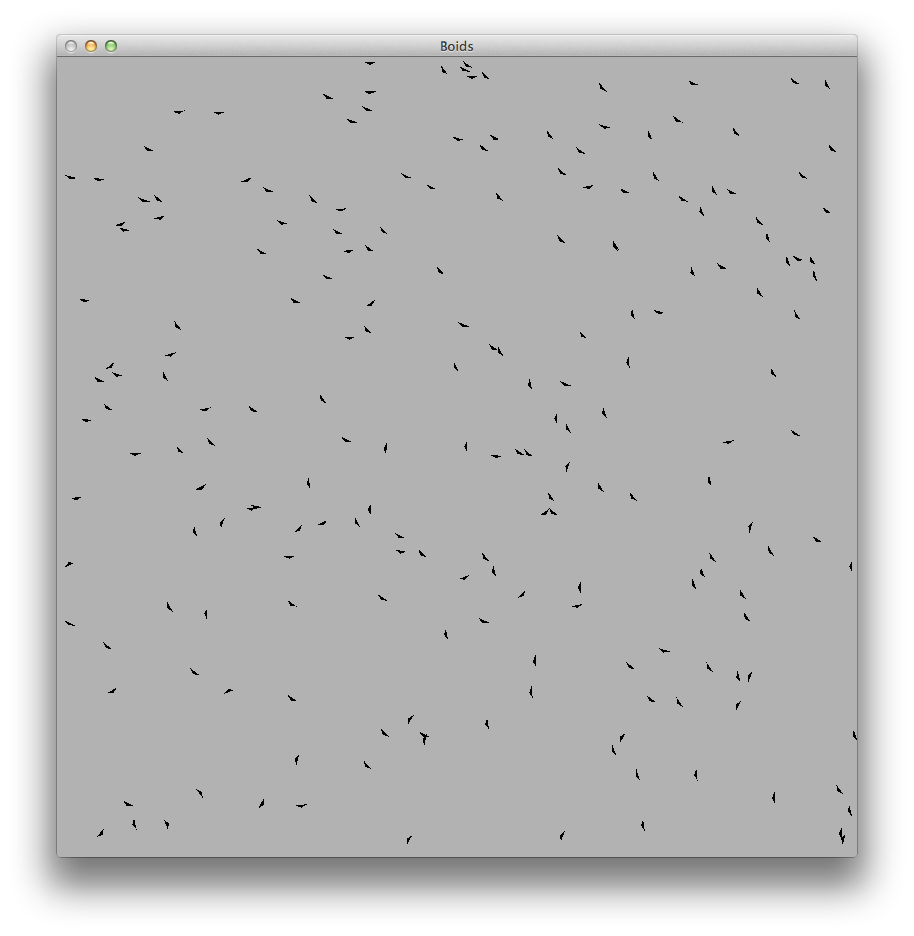
\includegraphics[width=0.5\textwidth]{assets/img/nodebug}
        \caption{Simulation run in swarm mode, with debugging off.}
        \label{fig:no-debug}
    \end{figure}
    
    \begin{figure}
        \centering
        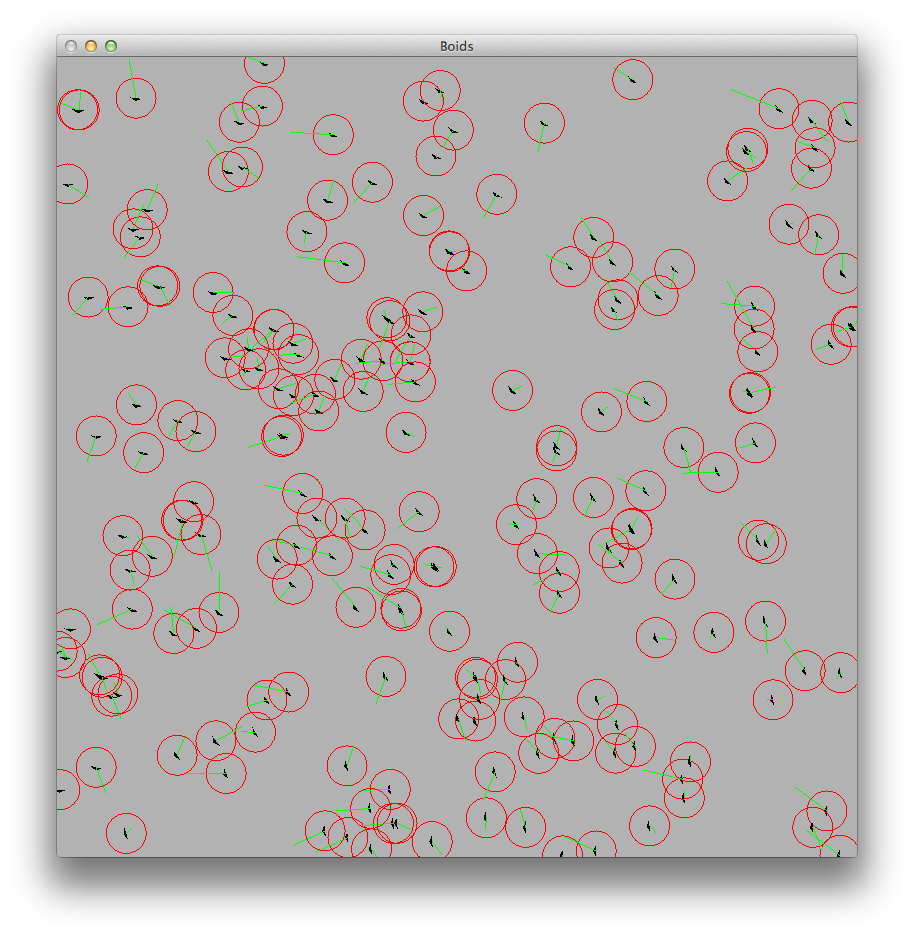
\includegraphics[width=0.5\textwidth]{assets/img/eqweight}
        \caption{Simulation run in equal-weight mode, with debugging and radii of size 20.}
        \label{fig:eqweight}
    \end{figure}
    
    \begin{figure}
        \centering
        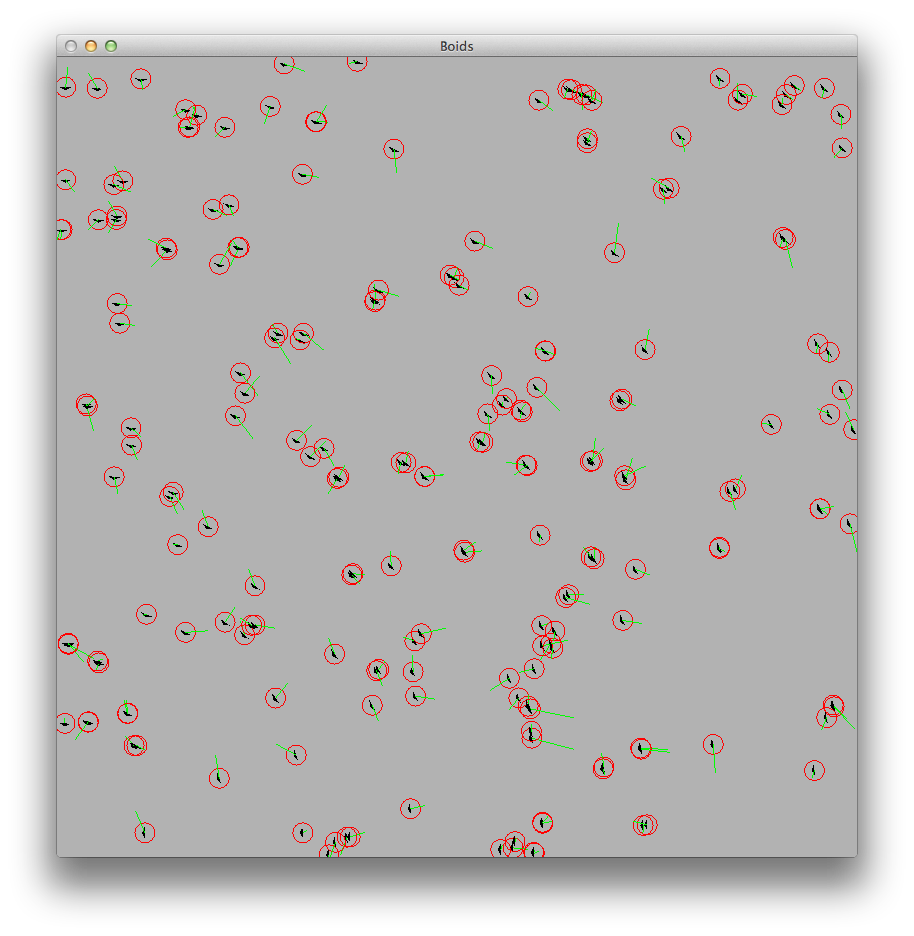
\includegraphics[width=0.5\textwidth]{assets/img/eqweight-small}
        \caption{Simulation run in equal-weight mode, with debugging and radii of size 10.}
        \label{fig:eqweight-small}
    \end{figure}
    
    \begin{figure}
        \centering
        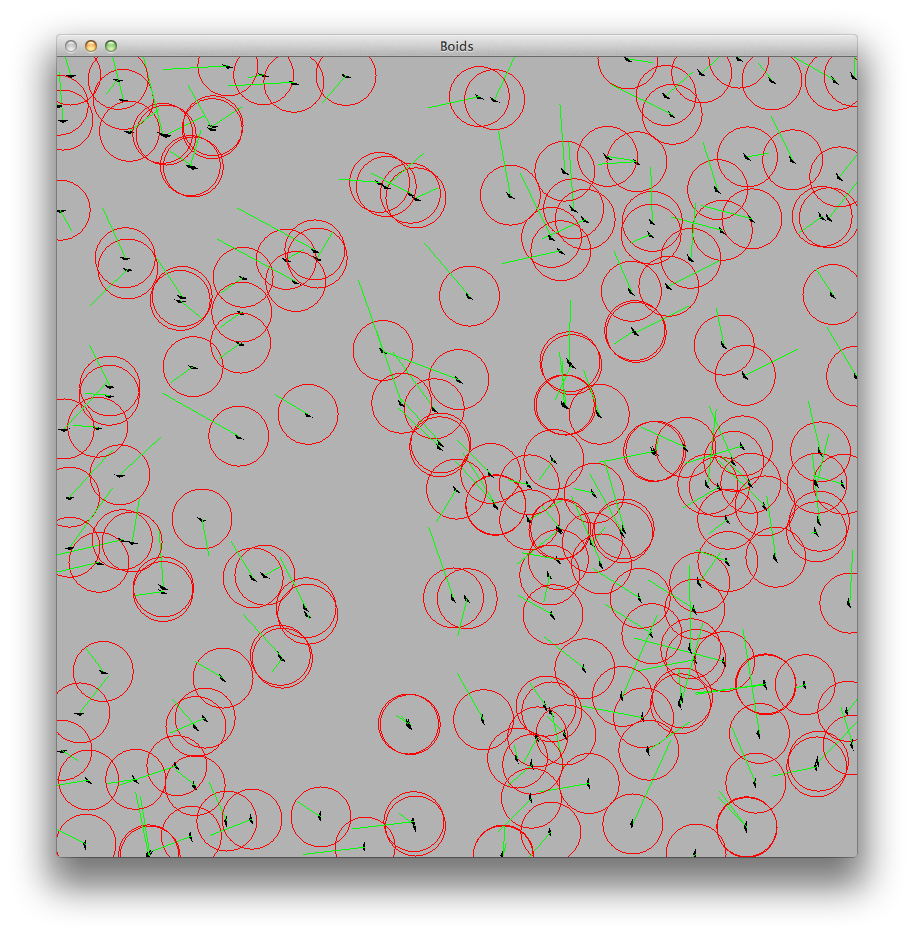
\includegraphics[width=0.5\textwidth]{assets/img/eqweight-large}
        \caption{Simulation run in equal-weight mode, with debugging and radii of size 30.}
        \label{fig:eqweight-large}
    \end{figure}
    
    \begin{figure}
        \centering
        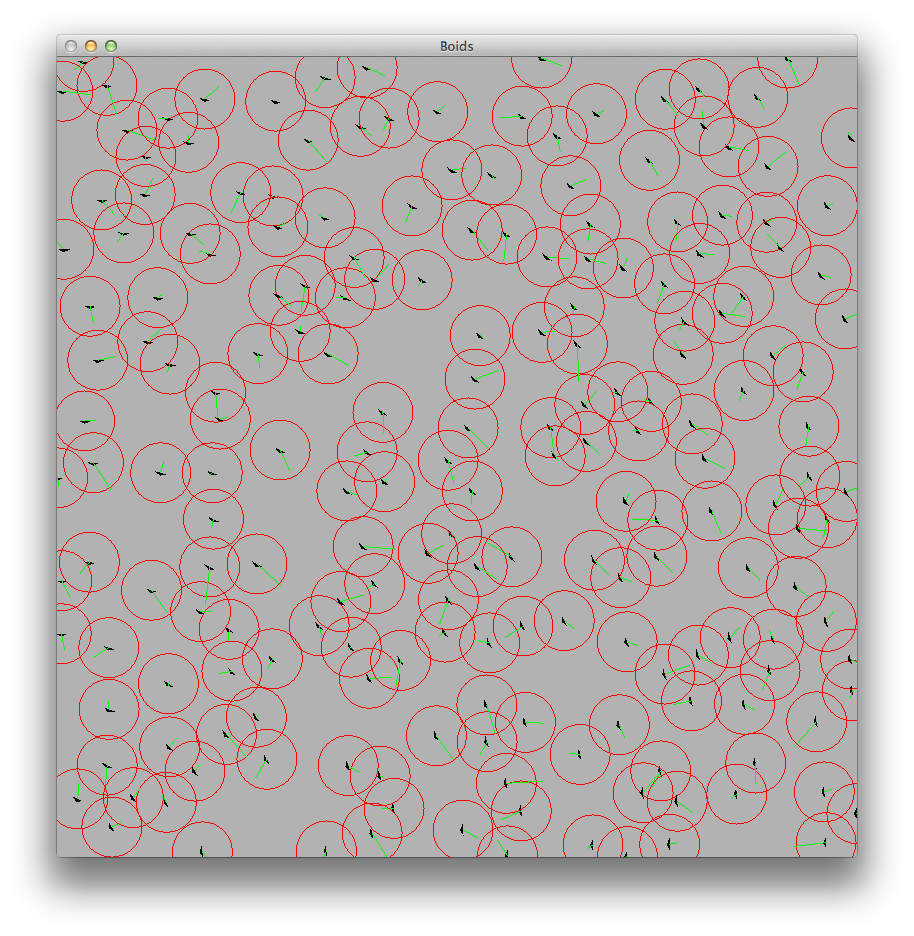
\includegraphics[width=0.5\textwidth]{assets/img/cohesion}
        \caption{Simulation run in cohesion mode.}
        \label{fig:cohesion}
    \end{figure}
    % describe behavior for each mode
    \FloatBarrier
\section{Conclusion}
    \subsection{Challenges}
    One of our major challenges was the existence of a bug in the ``alignment'' behavior of our code. This bug caused all boids in the scene to speed up erratically, eventually causing overflow in the vector components of the boids' velocities, and causing the program to crash. This was fixed after we realized that the neighborhood selection code for each boid included the boid itself, and thus added on the boid's own velocity to itself in the alignment function.
    \par Another challenge we faced early on was our early ambitions of creating a 3D simulation using the Haskell OpenGL bindings. These bindings caused us a number of problems, and abandoning them in favor of the 2D \texttt{gloss} library allowed us to focus on the details of our implementation with greater detail. Neither of us is particularly experienced with computer graphics, and we found that the higher level of abstraction provided by \texttt{gloss} made our task much easier. Furthermore, using OpenGL directly requires writing code that could be considered fairly unidiomatic in Haskell.
    
    \subsection{Takeaways}
    Both group members enjoyed the experience of implementing a multi-agent system using a purely functional programming language. As Hawk had significantly less experience programming in Haskell than Will, he found this assignment to be a particularly good learning experience in that language, but both members of the team enjoyed the opportunity to try something different than the previous course assignments. Furthermore, we found experimenting with Haskell's libraries for vector mathematics, as necessitated by the boids algorithm, to be interesting and fun.
    \par We also enjoyed being able to implement swarming and flocking behavior in a multi-agent system. Our previous experiences with swarming in class had only involved using preexisting programs, so we were interested in how such programs were written. Although Boids is not a particularly complex algorithm, the simulations it produces provide a fairly convincing approximation of real-life bird behavior. Both team members are very interested in `artificial life' simulations in general --- for his first final project in a computer science course at Allegheny, Will wrote an implementation of Conway's Game of Life in Processing. As this project is his last final project for a computer science course here at Allegheny, artificial life provides `book ends,' in a sense, on his Allegheny career.

\printbibliography

\end{document}